\chapter{Work Plan}\label{chap:workPlan}

\section{Approach and  Main Tasks}
Dwight Eisenhower, United States' President from 1953 to 1961 and Army Officer, said that `no battle was ever won according to plan, but no battle was ever won without one'. Hence, although this initial planning draft might not be religiously followed in all its extent, it is important to break down the work in \textbf{tasks} so that I and my supervisors can keep track of what has to be done, and establishing deadlines for the small achievements that, together, will build up to the succesful completion of the proposed work of this thesis. The detailed explanation of each task is provided in Section~\ref{sec:wp_tasks_td} and the \textbf{schedule} for them, where their approximate begin and end weeks are marked, is represented by a \emph{Gantt Chart} in Section~\ref{sec:wp_tasks_gantt}.

\subsection{Task Description}\label{sec:wp_tasks_td}
The work will be partitioned in \emph{five} large groups of tasks, and each of these groups will be further partitioned in smaller subtaskswhich are the actual assignements that I will be completing. We can think of the group of task as a sort of \emph{logical} grouping of the subtasks, according both to their relatedness and also to their precedence relationships. The task groups, and their related subtasks, are as follows

\begin{itemize}
    \item \textbf{T1 -- Preparation} -- This stage is the initial phase of the work, where I will essentialy setup my working environment and finish the Python modules for the LSTM network that will be used in the validation of my Verilog modules

        \begin{itemize}
            \item \textbf{T1.1 -- Complete Python Class with SPSA} -- here I will finish the Python modules that I have already developed as a preparation for this work, whose details are presented in Section~\ref{chap:earlyWork}, by adding the SPSA training algorithm, as opposed to the current Backpropagation Throgh Time version.

            \item \textbf{T1.2 -- Reproduce the Benchmark Results with the Python Class} -- after developing and testing the Python Class with SPSA, I will try to reproduce with it the results of~\cite{Tavear13}, in order for me to have a high-level model whose performance is comparable to~\cite{Tavear13, Hochreiter07}, and thus provide a good performance baseline for this and other future benchmark tests that I would like to run in order to compare my FPGA solution with a software solution.

            \item \textbf{T1.3 -- Setup FPGA Development Board} -- this is a farily technical step, where I setup my working environment, and make sure that everything is working correctly and is properly configured. As will be pointed out in Section~\ref{sec:wp_sh}, the FPGA development board of choice will be Xilinx~\textregistered Zedboard.

            \item \textbf{T1.4 -- Familiarize with the Zedboard} -- before any actual use, I should synthesize and run some sample designs, and perhaps write a small Verilog design, and go through the full design flow, from behavioural simulation, to synthesis. This will allow me to know exactly what steps to take when I will need to develop and test my Dissertation related modules, and focus more on the solving the problem at hand rather than solving technical details.
        \end{itemize}

    \item \textbf{T2 -- HDL Module Development} -- this is where I will port the ideas from Section~\ref{chap:theorBack} to fully functional HDL blocks, using Verilog and targeting a Zedboard technology.

        \begin{itemize}
            \item \textbf{T2.1 -- Design Planning} -- before performing and HDL coding, it is favourable to first assemble the system design strategy in paper. This is where, together with my supervisor, I will outline the internal organization of my system, and make the fundamental design decisions. Of course, this task will prolong during all the \textbf{T2} extent, since some design changes to the original plan will have to be performed as I find \emph{bugs} in my early Verilog implementations that force a design correction.

            \item \textbf{T2.2 -- Design SPSA Module} -- this task comprises the Verilog description of the module that will update the network weights using SPSA, and also the development of a testbench to validate my description. Furthermore, I will compare the output of this model with the golden output produced by a standalone SPSA Python Class previously developed in \textbf{T1}.
            \item \textbf{T2.3 -- Design LSTM Neuron/Layer Module} -- similar to the previous task, but now I am aiming to implement the actual LSTM Neuron or a layer of LSTM Neurons. This is a design decision that will need to be set in \textbf{T2.1}, to asses whether it is justifiable to have dedicated multiplication units assigned to each neuron, or we can perform matrix-like batch multiplications and treat the LSTM as a batch of Neurons, i.e. as a layer. Like in the previous task, a testbench will also be developed, and the module validate both with it and the Python golden output.

            \item \textbf{T2.4 -- Integrate and Validate both LSTM and SPSA modules} -- here, after the modules designed in \textbf{T2.2} and \textbf{T2.3} are validated individually, I will integrate them together in a higher level module, and perform a behavioural simulations of the new integrated module, as well as a verification procedure where the results from~\cite{Tavear13} will hopefully be reproduced and compared against the Python golden output.

        \end{itemize}

    \item \textbf{T3 -- FPGA Synthesis of the Verilog Code} -- after having Verilog code that passed all the validation tests and whose correct functionality is, therefore, asserted, I will synthesize the Verilog modules to FPGA RTL blocks, and perform a new simulation on these RTL syntesized code, that unlike the previous behavioural simulation, now has timing information resulting from the FPGA block mapping, and the place and routing of those mapped blocks.

        \begin{itemize}
            \item \textbf{T3.1 -- Synthesis of the SPSA Module} -- the module developed in \textbf{T2.2} is now syet
                {bar height=.6}thesized and validated
            \item \textbf{T3.2 -- Synthesis of the LSTM Neuron/Layer Module} -- same as the previous task, but now on the module of \textbf{T2.3}
            \item \textbf{T3.3 -- Integration of the Modules and Validation} -- the modules synthesized in the previous tasks are integrated and validated using the same testbench as in \textbf{T2.4}.
        \end{itemize}

    \item \textbf{T4 -- Benchmarking the Design} -- at this stage, we have a fully functional FPGA design of an LSTM network with SPSA on-chip training. Henceforth, we will need to benchmark its performance by comparing it to~\cite{Tavear13, Hochreiter07}, and prove its usefulness by using it in one or two usecases from~\ref{chap:stateArt}, which are interesting uses of Deep Learning techniques such as these.

        \begin{itemize}
            \item \textbf{T4.1 -- Benchmark the Performance/Computing Time} -- perform a side-by-side comparison of our model with the software counterpart of\cite{Tavear13, Hochreiter07} and with the only hardware implementation of LSTM of~\cite{Chang15}.
            \item \textbf{T4.2 -- Reproduce some of the state of the art applications of LSTM} -- in order to be able to show real-life, user-oriented, applications, I understand it is a good idea to try to reproduce some of the state of the art usages of LSTM, outlined in Section~\ref{chap:sa_apps}. It is too early to commit myself to which of these applications I will use, and how many, because that will depend on how well the work on tasks \textbf{T2} and \textbf{T3} is flowing. Nevertheless, I intend to at least impement one or two of them.
        \end{itemize}

    \item \textbf{T5 -- Write the Dissertation Final Report} -- while all the stages of work are developing, this task will obviously be active, by documenting all the design decisions, milestones acheieved and logging all the results that come from the implementation. A couple of weeks before the deadline, this will be the only active task, since producing a clear and well-written document requires concentration and undivided attention.

\end{itemize}

\subsection{Tentative Task Scheduling}\label{sec:wp_tasks_gantt}
Here is the Gantt Chart that depicts the temporal extension of the tasks described in Section~\ref{sec:wp_tasks_td}. 
\begin{landscape}
    
    \ganttset{bar height=.2}
    \ganttset{calendar week text= \small {\startday/\startmonth}}
    \begin{ganttchart}[vgrid, x unit=0.16cm, y unit chart=0.65cm, time slot format=isodate]{2016-02-15}{2016-06-26}

        \gantttitlecalendar{year, month, week} \\
        \ganttgroup{\textbf{T1}}{2016-02-15}{2016-02-29} \\
        \ganttbar{\textbf{T1.1}}{2016-02-15}{2016-02-22} \\
        \ganttbar{\textbf{T1.2}}{2016-02-22}{2016-02-29} \\
        \ganttbar{\textbf{T1.3}}{2016-02-15}{2016-02-22} \\
        \ganttbar{\textbf{T1.4}}{2016-02-22}{2016-02-29} \\

        \ganttgroup{\textbf{T2}}{2016-02-29}{2016-04-11} \\
        \ganttbar{\textbf{T2.1}}{2016-02-29}{2016-03-28} \\
        \ganttbar{\textbf{T2.2}}{2016-02-29}{2016-03-07} \\
        \ganttbar{\textbf{T2.3}}{2016-03-07}{2016-03-21} \\
        \ganttbar{\textbf{T2.4}}{2016-03-21}{2016-04-11} \\
        
        \ganttgroup{\textbf{T3}}{2016-04-11}{2016-05-02} \\
        \ganttbar{\textbf{T3.1}}{2016-04-11}{2016-04-18} \\
        \ganttbar{\textbf{T3.2}}{2016-04-18}{2016-04-25} \\
        \ganttbar{\textbf{T3.3}}{2016-04-25}{2016-05-02} \\

        \ganttgroup{\textbf{T4}}{2016-05-02}{2016-06-06} \\
        \ganttbar{\textbf{T4.1}}{2016-05-02}{2016-05-16} \\
        \ganttbar{\textbf{T4.2}}{2016-05-09}{2016-06-06} \\

        \ganttgroup{\textbf{T5}}{2016-02-29}{2016-06-26} \\

    \end{ganttchart}

\end{landscape}
\section{Software and Hardware resources to be used}\label{sec:wp_sh}

\subsection{Hardware Resources}
The main hardware resource that I will use for my solution is the \textbf{Xilinx\textregistered~ Zedboard} (Figure~\ref{fig:zedboard}, whose core is a Zynq-7000 System-on-Chip that features both an FPGA core and an ARM \textregistered~ Cortex\texttrademark~-A9 processor. It is an FPGA development board that features several I/O interfaces such as Etherner, HDMI output, VGA output, Audio IOs, USB and UART, among other capabilites, making it easy to prototype additional features to the core design (i.e. for building the note transcription system of~\cite{Bock12}, and to make it operate in real-time, I would need an audio input, which I can easily get from the Audio IO, without investing time in connecting the codec and programming the FPGA to interface it).

\begin{figure}
    \centering
    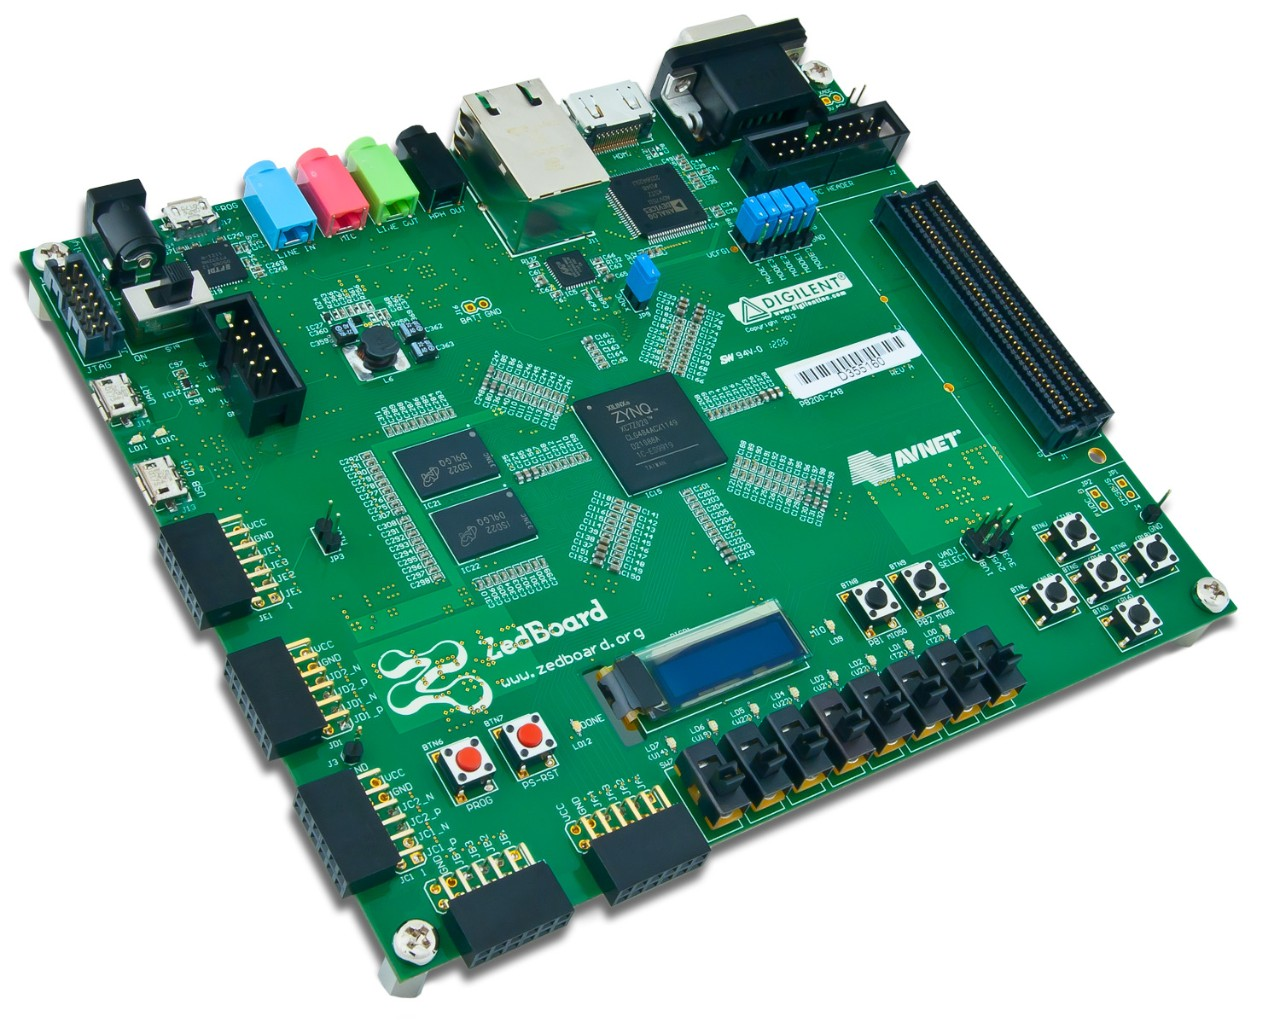
\includegraphics[width=\linewidth]{figures/zedboard.jpg}
    \caption{The Zedboard FPGA Development Board. Source: \href{http://www.xilinx.com}{Xilinx}}
    \label{fig:zedboard}
\end{figure}

\subsection{Software Resources}
In terms of software resources related to the FPGA development, I will need an \textbf{HDL simulation tool} to simulate and verify the Verilog code that I will develop, and a \textbf{Synthesis tool} to synthesize the Verilog files into RTL code, and to map that description into the resources available in the FPGA. The simulation tool used will be Questasim\texttrademark, the successor of the well-known Modelsim\texttrademark, which is an industry-standard tool in the area. For the synthesis tool, I will use Xilinx\textregistered Vivado Suite, also an industry-standard tool, and that is the only alternative, since the Zedboard is also produced by Xilinx\textregistered. These two tools are proprietary, but there are licenses available at FEUP. Furthermore, I am planning to use FloPoCo~\footnote{\href{http://flopoco.gforge.inria.fr/}{http://flopoco.gforge.inria.fr/}} to generate some of the modules that perform arithmetic operations, to hasten the developing effort/time, and to ensure that they are the most efficient possible, and don't pose a performance bottleneck to my design; this software is freeware, and a standard in Academia.

For the Python Classes, I will make use of the 3.3 version of the Python distribution, the high-performance numerical computation library Numpy\footnote{\href{http://www.numpy.org/}{http://www.numpy.org/}}, which is a standard in scientific computing, and the Matplotlib\footnote{\href{http://matplotlib.org/}{http://matplotlib.org/}} plotting library. All of this software is also free to use, and open-source. I may also need to use the PyBrain\footnote{\href{http://pybrain.org/}{http://pybrain.org/}} framework, since it has an LSTM implementation. 

To write the final Disseration report, I will use \LaTeX (this report itself was also written in \LaTeX), and mostly use Tikz, Inkscape and Matplotlib to produce figures and drawings. Once again, all of this is free to use.
